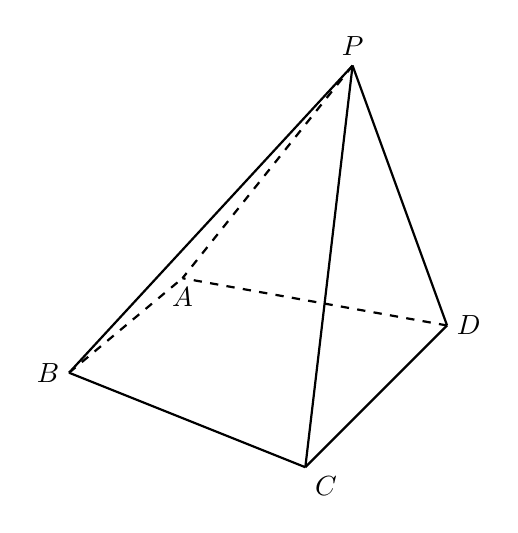
\begin{tikzpicture}[scale=1.2, line join=round]
    % 1. 定义底面与顶点的二维投影坐标
    \coordinate (A) at (1.2, 1.5);
    \coordinate (B) at (0, 0.5);
    \coordinate (D) at (4, 1);
    \coordinate (C) at (2.5, -0.5);
    \coordinate (P) at (3, 3.75);

    % 2. 绘制不可见的虚线边
    \draw[dashed, thick] (P) -- (A);
    \draw[dashed, thick] (B) -- (A);
    \draw[dashed, thick] (D) -- (A);

    % 3. 绘制可见的实线边
    \draw[thick] (P) -- (B);
    \draw[thick] (P) -- (C);
    \draw[thick] (P) -- (D);
    \draw[thick] (B) -- (C);
    \draw[thick] (C) -- (D);

    % 4. 标注顶点
    \node[below] at (A) {$A$};
    \node[left] at (B) {$B$};
    \node[below right] at (C) {$C$};
    \node[right] at (D) {$D$};
    \node[above] at (P) {$P$};

\end{tikzpicture}